\chapter{Bilder}

Um Bilder in \LaTeX{} einzufügen wird der Befehl \verb|\includegraphics[Option]{Pfad/Dateiname}| genutzt. Näheres zu dem Befehl hier: \url{http://www.golatex.de/wiki/%5Cincludegraphics}

Diese Optionen sind nur verfügbar, wenn zuvor das graphicx-Paket eingebunden wurde. Andere Pakete wie graphics unterstützen nicht alle Optionen.	
\begin{itemize}
\item angle - Bestimmt den Drehwinkel um einen Referenzpunkt für die Grafik. Positive Werte drehen die Grafik gegen den Uhrzeigersinn, negative mit ihm.
\item draft - Ist draft gesetzt, wird nur ein Platzhalter der Grafik angezeigt. Beschleunigt den Übersetzungsvorgang des Dokuments erheblich. Oftmals kann draft auch in den Dokumentoptionen angegeben werden.
\item scale - Skaliert die Grafik anhand eines Skalierungsfaktors.
\item height - Skaliert die Grafik auf die angegebene Höhe. Die Angabe der Größe muss in einer LaTeX-spezifischen Einheit erfolgen.
\item width - Skaliert die Grafik auf die angegebene Breite. Die Angabe der Größe muss in einer LaTeX-spezifischen Einheit erfolgen.
\end{itemize}	
% Wie fügt man Bilder ein
	% Wie muss Caption gemacht werden bzw. keine Caption
% Wie bekommt man Bilder nebeneinander
% Wie bekommt man Bilder umflossen vom Text

\begin{figure}[ht]
	\centering
	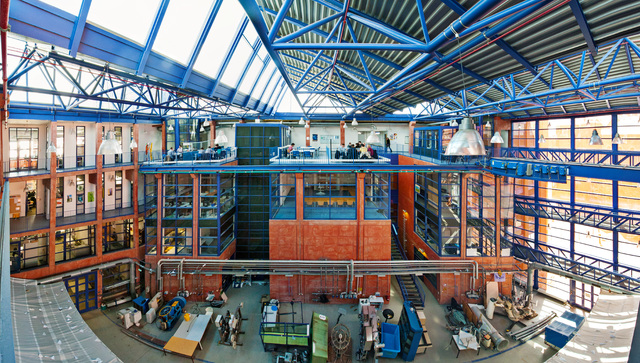
\includegraphics{images/Haus_Z.jpeg}
	\caption{Innenraum von Haus Z \cite{hauszpic}}
	\label{fig1}
\end{figure}

\verb|\includegraphics| muss nicht zwingend in einer figure-Gleitumgebung verwendet werden, ratsam ist es aber schon, da sonst keine Bildunterschriften bzw. Bezeichner gesetzt werden können. Die Bildunterschriften haben dabei immer unter dem Bild zu sein mit einem \verb|\cite{text}| auf den Ursprungsort des Bildes. Der Befehl \verb|\cite{text}| greift auf die \emph{.bib} Datei über den Bibtexkey zu. Weitere Informationen zur figure-Gleitumgebung finden sie hier: \url{https://en.wikibooks.org/wiki/LaTeX/Floats,_Figures_and_Captions}\newline

Auch Bilder können nebenbeinander platziert werden. Dies kann auf sehr verschiedene Weise erreicht werden: \url{http://texwelt.de/wissen/fragen/18877/zwei-bilder-nebeneinander-jeweils-mit-bildunterschrift-und-label} 

Als Beispiel wird in diesem Dokument das Paket \emph{floatrow} genutzt.
\begin{quote}
	"'Das Paket floatrow bietet zwei Features, die für die Umsetzung der Anforderung verwendet werden können.
	
	Zum einen kann man mit \verb|\ffigbox| eine Abbildung zusammen mit ihrer Bildunterschrift in genau der Breite setzen, die durch die Abbildung vorgegeben wird. Das funktioniert auch dann noch, wenn die Bildunterschrift mehrzeilig wird. Dazu ist als optionales erstes Argument \verb|\FBwidth| anzugeben. Als zweites Argument wird \verb|\caption[…]{…}| zusammen mit einem ggf. zu setzenden \verb|\label{…}| angegeben. Das dritte Argument ist die Abbildung.
	
	Desweiteren bietet das Paket die Möglichkeit, durch \verb|\ffigbox| angegebene Abbildungen innerhalb einer floatrow-Umgebung in Spalten nebeneinander anzuordnen. Für zwei Abbildungen nebeneinander muss man die beiden durch \verb|\ffigbox| definierten Abbildungen also nur zusätzlich in eine floatrow-Umgebung packen."'\cite{floatrow}
\end{quote}
\begin{figure}[h]
	\centering
	\begin{floatrow}
		\ffigbox[\FBwidth]{%
			\caption{Linke Abbildung}\label{fig:left}
		}{%
			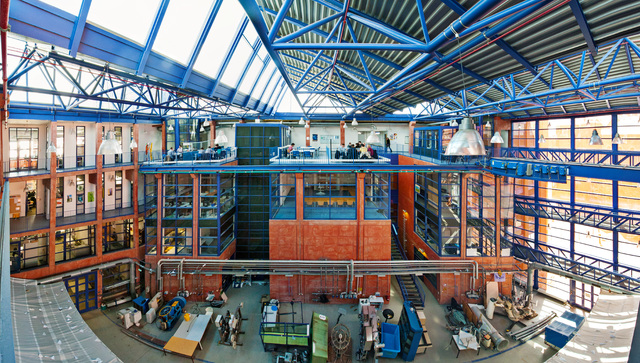
\includegraphics[scale=1]{images/Haus_Z.jpeg}
		}%
		\ffigbox[\FBwidth]{%
			\caption{Abbildung rechts neben der linken Abbildung}\label{fig:right}
		}{%
			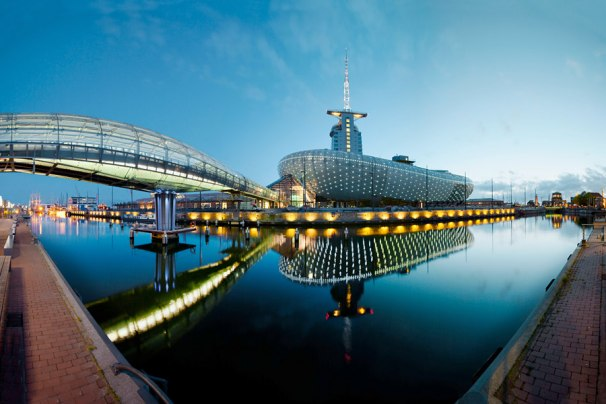
\includegraphics[scale=.3]{images/Klimahaus.jpeg}
		}%
	\end{floatrow}
\end{figure}

Um Bilder in einem Text zu platzieren sodass das Bild davon umschlossen wird, muss eine \verb|\wrapfigure| Umbegung genutzt werden.\\

\verb|\begin{wrapfigure}[Zeilen]{Position}[Ueberhang]{Breite}|\\
Um das Margin als den weißen Rand um das Bild zu reduzieren wird der Befehl \verb|\columnsep| des Paketes genutzt. Durch den Befehl \verb|\lipsum| erzeugt man Lorem Ipsum Text.\\

\lipsum[1-1]
\begingroup
\setlength{\columnsep}{-30pt} % verändert die Größe des Margin nach links und rechts
\setlength{\intextsep}{1pt}  %verändert die Größe des Margin nach oben und unten
\begin{wrapfigure}{R}{.6\textwidth}
	\begin{center}
		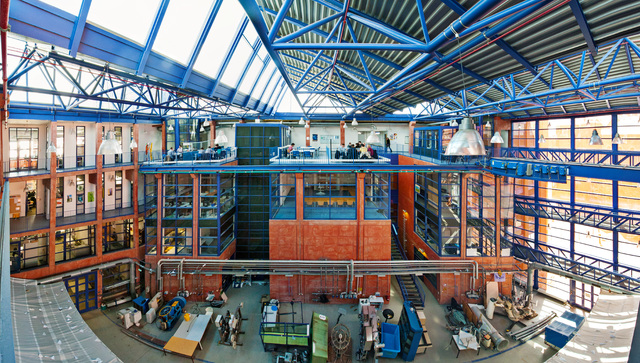
\includegraphics[width=0.6\textwidth]{images/Haus_Z.jpeg}
	\end{center}
	\caption{Rechtsbündig im Text \cite{hauszpic}}\label{fig:classrr}
\end{wrapfigure}
%\lipsum[1-1]
Dies asdhkajsdhak shaudhasi dhasidh aipudh aipsudhai sdh aipdh aipsdhapi dugh aipdh aipdh aipsudg asipd gauidg aipdgaipdg apid gaipg aif gsipf as pifg wizf a wui fais fis ufpsiudfsi df sipduf siu fsid uf si f spi fgsiufgsiufgsidufgsdidufgsipdufsiufbsiufsidufsidufhsiufhsidofhisdouisufhsidu  sidufh sdiufzsdi ufzsdiüufz sdiuü fzsdz fdsiufz dsiu fzsdiufz sdiu fzsduifsudi zfsduifz sud9f zsüdu füdsif asdjaköjsdnökajsdnökajsdhökajsdbnköajjs a shdpahs dpiau sdh ipau sdhpia hsdiüoau hd piausdh piausdg piagdipasudghipaushd piausdhpiaus de.
%Man benötigt bei \endgroup eine Leere Zeile zwischen Text und dem Befehl oder man nutzt \par
\par
\endgroup




